\documentclass[tikz,border=3pt]{standalone}
\usepackage{amsmath}
\usepackage{tikz}
\usepackage{pgfplots}
\pgfplotsset{compat=1.18}
\begin{document}
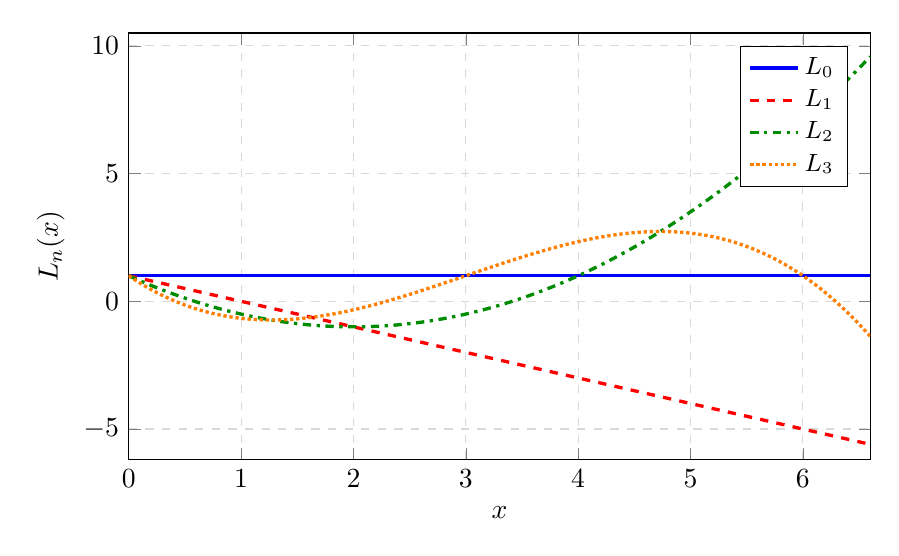
\begin{tikzpicture}
\begin{axis}[
  width=11cm, height=7cm,
  xlabel={$x$}, ylabel={$L_n(x)$},
  xmin=0, xmax=6.6, ymin=-6.2, ymax=10.5,
  legend style={at={(0.97,0.97)}, anchor=north east, font=\small},
  grid=both, grid style={dashed, gray!30},
  domain=0:6.6, samples=260,
  no marks
]
  \addplot[blue, very thick, solid] {1};
  \addlegendentry{$L_0$}
  \addplot[red, very thick, dashed] {1-x};
  \addlegendentry{$L_1$}
  \addplot[green!55!black, very thick, dashdotted] {1-2*x+x^2/2};
  \addlegendentry{$L_2$}
  \addplot[orange, very thick, densely dotted] {1-3*x+1.5*x^2-x^3/6};
  \addlegendentry{$L_3$}
\end{axis}
\end{tikzpicture}
\end{document}
